\chapter{Model Description}
\label{ch:model}

The model attempts to recreate a microgrid which uses some form of DER as a primary power source along side energy storage in order power the load. \autoref{fig:abridged_flow_diagram_label} shows a simplified flow diagram of the model using an ORC for the DER. The components include a ORC as a source, a load, and an inverter to link the source two. In the figure, the blue lines represent electrical connections, while green represents the flow of data and component parameters. The ORC block is made up of heat exchangers, an isentropic pump, an isentropic expander, and an induction generator. 
\begin{comment}
The load block \verb|one line description of load|. 
The energy storage block \verb|one line description of energy storage|. 
The inverter block \verb|one line description of inverter|.
\end{comment}
\begin{figure}[h]
	\centering
	\caption{A simplified diagram of power and data flows of the model. Blue lines represent electrical power connections and flows similar to a one-line diagram. Green boxes represent data flow from one part of the model to another.}
	\label{fig:abridged_flow_diagram_label}
	
	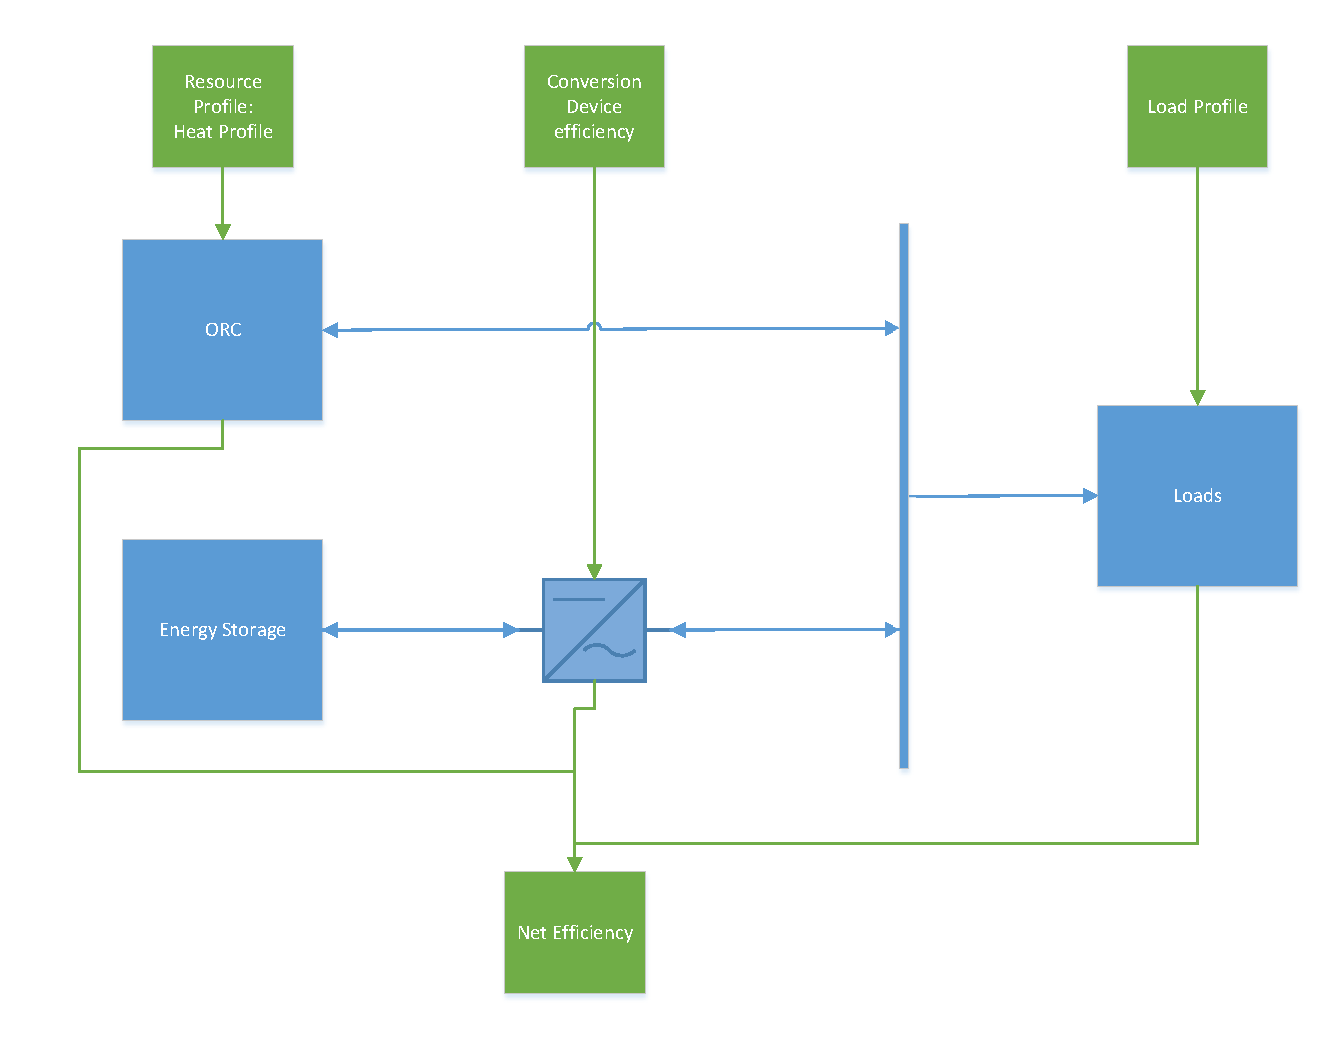
\includegraphics[width=\textwidth]{figures/Abridged Pilgrim Model Flow diagram - AC bus.pdf} 
	%\includegraphics[width=\textwidth]{figures/SimpleFlowDiagram.pdf}

\end{figure}

\section{Organic Rankine Cycle Generator}
The ORC generator block links the thermal, mechanical, and electric components of them model. The thermal properties of the fluids were obtained from a Matlab wrapper of the CoolProp library. \cite{Bell2014} Thermal conditions of source, sink, and working fluids are fed into the Rankine Cycle portion of the model, which returns a mechanical power. Electrical conditions, along with the mechanical power, are fed into the generator portion of the model, which returns an electrical output.  

\subsection{Evaporator and Condenser}
The evaporator and the condenser are both represented using a heat exchanger script.  The function takes as inputs parameters about the high and low temperature fluids, specifically the inlet temperatures or enthalpies (\si{\kelvin} or \si{\joule\per\kilogram}), mass flow rates (\si{\kilogram\per\second} ), inlet pressures (\si{\pascal}), and fluid names, as well as parameters about the exchanger itself such as the overall heat transfer coefficient (\si{\watt\per\kelvin\per\meter\squared}), the heat transfer area (\si{\meter\squared}), and the heat exchanger type (e.g. counter or parallel flow). The function output is made up of the heat flow rate (\si{\watt}), and the temperatures or enthalpies at the outlets (\si{\kelvin} or \si{\joule\per\kilogram}). 

In order to calculate the desired values, the Number of Transfer Units (NTU) method is used. Described in The Fundamentals of Heat and Mass Transfer, \cite{Incropera} this process calculates the output heat flow, $\dot{Q}$, relative to a theoretical maximum heat flow, $\dot{Q}_{max}$. This potential heat flow would be realized using an infinitely long counter flow geometry and is calculated as
\begin{equation}
\dot{Q}_{max} = C_{min}\left(T_{h,i} - T_{c,i}\right)
\end{equation}
where $C_{min}$ is the smaller heat capacity rate of the hot and cool fluids and $T_{h,i}$ and $T_{c,i}$ are the inlet temperatures of hot and cool fluids respectively. The heat capacity rate is the product of mass flow rate, $ \dot{m} $, and the mass specific heat at constant pressure, $ c_p $. 

The heat flow rates of the hot and cool fluids are related by the effectiveness, $\epsilon$, which is defined as 
\begin{equation}
\label{eq:effectiveness_def}
\epsilon \equiv \frac{\dot{Q}}{\dot{Q}_{max}}
\end{equation}

Numerically, the value of $\epsilon$ is a function of the ratio of the fluids' heat capacities, $C_r = \frac{C_{min}}{C_{max}}$, as well as the exchanger's Number of Transfer Units, $NTU = \frac{U \cdot A}{C_{min}}$, where $U$ is the overall heat transfer coefficient and $A$ is the total heat transfer area. Additionally, the direction of fluid flow changes the method of calculation. In parallel flow heat exchangers, the effectiveness is calculated as
\begin{equation}
\epsilon = \frac{1 - \exp\left[-NTU\left(1 + C_r\right)\right]}{1 + C_r}
\end{equation}
while counter flow devices use
\begin{equation}
\epsilon = \frac{1 - \exp\left[-NTU\left(1 - C_r\right)\right]}{1 - C_r\exp\left[-NTU\left(1 - C_r\right)\right]}
\end{equation}

Once the effectiveness and maximum heat transfer rate are determined, equation \ref{eq:effectiveness_def} is used to calculate the actual rate of heat flow, $\dot{Q}$. Finally, the change in temperature for each fluid is calculated based on their respective heat capacity rates at initial conditions and the rate of heat flowing between them. 
If the change in temperature for either fluid would result in vaporization or condensation, then the values must be recalculated because the specific heat is effectively infinite while the fluid is changing states. 

First, the heat flow rate necessary to have the fluid begin changing its state is determined and the fraction of this value relative to initial heat flow rate is calculated. 
The heat transfer area is reduced by this fraction and the function is re-run inputing the state of the two fluids as the one fluid begins to change phase. If enough heat flows between the two fluids such that the one completes the phase change, then the function is run a third time with the heat transfer area modified again. 

Within this script there are certain assumptions made in order to calculate the output values. The function will not return accurate results if both fluids simultaneously undergo a phase change because the ratio of heat capacities, $C_r$, will be undefined. Additionally, Ambient temperature and associated heat flow to the external environment is not accounted for in the script. Finally, it is assumed the pressure drop from inlet to outlet is negligible for both the high and low temperature fluids. 

\subsection{Expander and Pump}
The expander/turbine and pump components are both modeled by a fluid undergoing non-ideal isentropic expansion or compression. For an ideal isentropic process, the fluid will experience some thermodynamic changes while its internal entropy remains constant. 

The function takes as inputs certain properties of the fluid, such as the inlet temperature or enthalpy (\si{\kelvin} or \si{\joule\per\kilogram}), both the inlet and outlet pressures (\si{\pascal}), and the mass flow rate (\si{\kilogram\per\second}). Also needed is the isentropic efficiency, a unitless parameter of the machine which describes lost power due to deviations from the ideal insentropic process. The function returns the power produced or consumed\footnote{Power is produced if the pressure at the inlet is greater than at the outlet, and consumed if inlet pressure is less than that of the outlet.} (\si{\watt}) and the temperature or enthalpy (\si{\kelvin} or \si{\joule\per\kilogram}) of the fluid at the outlet.

Using the inputs and the Cool Prop library, the Mass Specific Entropy, $S$, of the fluid is determined for the fluid at the inlet. In an ideal process, this value would remain constant, so it is used to determine the ideal enthalpy of the outlet. Next the ideal power transferred is calculated as 
\begin{equation}
\label{eq:power_enthalpy}
P = \dot{m} \left(H_i - H_o\right)
\end{equation}
where $H_i$ and $H_o$ are the inlet and outlet enthalpies respectively.

To obtain the mechanical power actually transferred, the isentropic efficiency is applied to the ideal power such that the ideal is necessarily greater than the actual. When the value of $H_i$ is larger than $H_o$, $P$ is positive therefore efficiency is multiplied. When $H_i$ is less than $H_o$, $P$ is negative and ideal power is divided by efficiency. After the mechanical power is calculated, equation \ref{eq:power_enthalpy} is used to find $H_o$ and the fluid temperature at the outlet. 

\subsection{Induction Generator}
The generator block models a Squirrel Cage Induction Generator (SCIG) in order to convert the mechanical power to an electrical form. Two different function blocks were created for two scenarios: regulated and unregulated. The former is simpler to model, but the generator requires another firm source\footnote{Or an electrical storage-inverter combination.} to maintain its frequency and voltage. For the latter scenario, the generator's frequency and voltage are allowed to vary. Its leads are connected directly to a power converter which maintains the frequency and voltage of the remaining microgrid. 

\subsubsection{Regulated SCIG}
This function block takes several electrical and mechanical parameters as inputs such as the line to line voltage (\si{\volt}) and electrical frequency (\si{\hertz}) at the leads, the mechanical speed at the shaft (\si{\rpm}), the number pole pairs in machine's windings, and coefficients of friction due to bearings (\si{\watt\per\second}) and windage (\si{\watt\per\second\squared}). Also input are the resistive and inductive impedances (\si{\ohm}) of the stator, rotor, and core, as well as the capacitive impedance and equivalent series resistance of external excitation capacitor. The function returns the active (\si{\watt}) and reactive (\si{\voltampreactive}) power outputs and losses.

\begin{figure}[h]
	
\centering

\begin{tikzpicture}[american voltages]
\draw[color=black, thick]
%Input
(0,0) to [open, l=$V_{ph}$, o-o] (0,4){}

%low
(0,0) -- (9,0){}

%stator
(0,4) -- (1.5,4) to [R, l=$R_{s}$] (3,4) to [L, l = $j X_{s}$] (4.5,4){}

%rotor
(4.5,4) -- (5.5,4) to [R, l=$R_{r}$] (7.5,4) to [L, l = $j X_{r}$] (9,4) to [R, l=$R_{r}\frac{1-s}{s}$] (9,0){}

%core
(5,4) to [short, *-*] (5,3){}
(4.5,3) -- (5.5,3) to [L, l = $j X_{m}$] (5.5,1) -- (4.5,1) to [R, l=$R_{c}$] (4.5,3){}
(5,1) to [short, *-*] (5,0){}

%external excitaion capacitor
(1,4) to [R, l=$R_{esr}$, *-] (1,2) to [C, l=$-j X_x$] (1,0.5) to [short, -*] (1,0){}


;
\end{tikzpicture}

\caption{Single phase diagram of a three phase squirrel cage induction machine. $V_{ph}$ and $s$ are the phase voltage and slip of the generator. }
\label{fig:SCIG__circuit_diagram}

\end{figure}
A single phase circuit diagram of the generator which includes these components can be seen in \autoref{fig:SCIG__circuit_diagram}. $R_s$ and $X_s$ represent the resistive and inductive impedances of the stator. $R_r$ and $X_r$ represent the resistive and inductive impedances of the rotor as referred to the stator. $R_c$ and $X_m$ represent the resistive and inductive impedances due to the magnetization of the core. $R_{esr}$ and $X_x$ represent the equivalent series resistance and capacitive impedances of the external excitation capacitor.

To calculate these outputs, first the magnitude of the phase voltage is determined from the line to line voltage, $V_{ll}$, as $ \left|V_{ph}\right| = \frac{\left|V_{ll}\right|}{\sqrt{3}} $ assuming $ \angle V_{ph} = 0\deg $. Next the synchronous mechanical speed is determined by $ n_{synch} = \frac{120f}{2\text{poles}} $ and is used, along with the mechanical speed, $n_{mech}$ to calculate the slip of the machine as $ s = \frac{n_{synch} - n_{mech}}{n_{synch}} $.

The impedances of the stator, rotor, core impedances, the Th\'evenin combination of those three branches, the external excitation branch, and the Th\'evenin combination of all branches are calculated as
\begin{equation*}
Z_s = R_s + jX_s
\end{equation*}
\begin{equation*}
Z_r = R_r\frac{1-s}{s} + R_r + jX_r
\end{equation*}
\begin{equation*}
Z_{core} = R_c \parallel jX_m
\end{equation*}
\begin{equation*}
Z_{machine} = R_s + \left(Z_{core} \parallel Z_r\right)
\end{equation*}
\begin{equation*}
Z_{excite} = R_{esr} - jX_x
\end{equation*}
\begin{equation*}
Z_{total} = Z_{excite} \parallel Z_{machine}
\end{equation*}

Once all the relevant impedances are determined, the currents flowing through the branches are calculated along with the internal voltage at the stator-rotor-core junction. These values are used to determine internal power losses. The mechanical losses due to the bearings and windage are calculated by multiplying the appropriate coefficient of friction by the mechanical angular frequency  and the square of the mechanical angular frequency respectively. 

\subsubsection{Unregulated SCIG}
To simulate microgrids with no forms of storage or sources beyond the ORC, an unregulated SCIG model was developed. The single phase diagram is similar to the regulated SCIG seen in \autoref{fig:SCIG__circuit_diagram}, except the voltage source $V_{ph}$ at the lead is replaced with a resistive load. The model is based off the analysis by Ouazenne et al. of a self excited induction generator in \cite{Ouazenne1983} using admittance balancing. It is assumed the active power losses across the core and the excitation capacitance are negligible. Additionally, it is assumed the load is purely active, as any reactive load can be supplied by the conversion device which regulates the voltage and frequency of the microgrid.

The method of admittance balancing relies on the fact active and reactive power entering and exiting an electrical node must sum to zero. For this analysis, the chosen node at which the rotor, the core, and the combination of the stator, excitation capacitor, and load meet. Since the voltage across each branch is the same and power flow sums to zero, then the admittances must sum to zero as well. By breaking the complex admittances into real and imaginary components, a system of equations can be developed to solve for frequency and core reactance. 
%A more detailed description of this process can be seen in Appendix \autoref{ap:SEIG}. 
These values can then be used to determine total power output and losses. 

The function takes as variable inputs the mechanical speed of the shaft (\si{\rpm}), the power load of the microgrid (\si{\watt}), and the line to line voltage at the lead (\si{\volt}). Also input as parameters are the rated frequency of machine (\si{\hertz}), the number of poles it contains, the resistances and inductances of the rotor and stator (\si{\ohm}, \si{\henry}), the capacitance of external excitation capacitors (\si{\farad}), coefficients of friction due to bearings (\si{\watt\per\second}) and windage (\si{\watt\per\second\squared}), and the magnetization curve comparing the core reactance (\si{\ohm}) to the internal voltage across the core (\si{\volt}). The output variables of the function include active power generated (\si{\watt}) and internally consumed (\si{\watt}), the reactive power consumed (\si{\voltampreactive}), the necessary mechanical power driving the shaft (\si{\watt}), the line to line voltage (\si{\volt}), and the electrical frequency (\si{\hertz}).

First the inductive and capacitive reactances of the rotor, stator, and external excitation capacitors are calculated at the rated frequency of the machine, along with the equivalent load resistance for the given input voltage. Next, the electrical frequency is calculated based off the real portion of the admittance balance equations. With the frequency the machine slip can be determined as well. Next, the imaginary portion of the admittance balance equation can be used to solve for the core reactance. Internal voltage of the machine is then interpolated from the core reactance based off of the magnetization curves. The new line voltage is determined as well to feed back into the next iteration of the function.

With all components of the machine known, the power output and losses can be calculated in the same manner as the regulated induction generator seen above. The power generated is fed into the input of the inverter block and the losses are used in the feedback control.

\section{Inverter}
The inverter block converts the unregulated power output from the generator into a form with a stable frequency and voltage. In this model, a simplified view is taken of its operation. The inputs include the inverter's efficiency, $\eta$, and the unregulated power off of the induction generator (\si{\watt}). The outputs include the delivered power to the load calculated as $P_{out} = \eta P_{in}$  and the power lost within the inverter (\si{\watt}) calculated as $P_{loss} = P_{in} - P_{out}$. 

\section{Load}
The model is assumes the microgrid delivers power to a three-phase \SI{60}{\hertz} AC load. The total load in the model is determined by the sum of a predefined set point and the power consumed by the pump used to circulate the working fluid. The electrical power of the pump is determined by dividing the mechanical power output of pump function by the efficiency of the pump driver. In addition to the active load, it is assumed there is a reactive load determined by a predefined power factor parameter. 
The load seen by the unregulated induction generator is the sum of the total load and the losses due to the inverter. 

The total load is combined with both the inverter and generator losses in order to provide the reference of a PI controller. The sum is then compared to the output mechanical power of the ORC system. A gain is applied to the error signal and integrated to provide the desired flow rate of the working fluid. The gain value was selected in order to quickly reach steady state during the simulation.

\section{Validation}
Before simulating  the greenfield and brown field scenarios, the model needs to be validated. This is done using the results of an ORC test at the University of Alaska Fairbanks conducted in 2013 \cite{Lin2014}. The report details the process of testing an Electratherm Green Machine ORC system in a controlled environment at the UAF power plant and in the field for waste heat reclamation of a diesel generator at the Tok, Alaska powerhouse.

During the sizing of the ORC system turbine and pump efficiencies as well as heat exchanger areas and transfer coefficients were assumed based off publications and conventional practice, but final values were not reported. These assumed values are used as the input of the model. All of the non-variable ORC parameters for the validation can be seen in \autoref{tab:verification_ORC_params}.
\begin{table}%[h]
	\centering
	\caption{Input parameters for the validation of the ORC prime power system model.}
	%\rowcolors{5}{}{gray!10}
	\label{tab:verification_ORC_params}
	\begin{tabular}{rl}
		\toprule
		           Parameter & Value                                        \\ \midrule
		         $U_{evap}$ & 1500 \si{\watt\per\kelvin\per\meter\squared} \\
		         $A_{evap}$ & 26.5 \si{\meter\squared}                     \\
		         $U_{cond}$ & 1400 \si{\watt\per\kelvin\per\meter\squared} \\
		         $A_{cond}$ & 102.5 \si{\meter\squared}                    \\
		    $\eta_{turbine}$ & 0.78                                         \\
		       $\eta_{pump}$ & 0.7                                          \\
		$\eta_{pump\ driver}$ & 0.9                                          \\
		   $\eta_{inverter}$ & 1.0                                          \\ \bottomrule
	\end{tabular}
\end{table}


The only reported electrical parameters of the three-phase induction generator were the frequency (\SI{60}{\hertz}), and the voltage (\SI{480}{\volt}). The impedance parameters were taken from a 10 HP machine in \cite{Ouazenne1983} and scaled based off the expected relative power output. The external excitation capacitance was selected in order to yield a terminal voltage roughly equal to the rated voltage. The impedance parameters can be seen in \autoref{tab:verification_SCIG_params}.
% and the magnetization curve comparing internal voltage, $E$, and the magnetizing reactance at rated frequency, $X_m$, can be seen in Fig X.
\begin{table}%[h]
	\centering
	\caption{Input generator parameters for the validation of the organic Rankine cycle prime power system model.}
	%\rowcolors{5}{}{gray!10}
	\label{tab:verification_SCIG_params}
	\begin{tabular}{rl}
		\toprule
		    Parameter & Value                                       \\ \midrule
		      $poles$ & 4                                           \\
		  $f_{rated}$ & $\SI{60}{\hertz}$                           \\
		        $R_s$ & $\SI{0.0279}{\ohm}$                         \\
		        $X_s$ & $\SI{0.0798}{\ohm}$                         \\
		        $R_r$ & $\SI{0.0272}{\ohm}$                         \\
		        $X_r$ & $\SI{0.0475}{\ohm}$                         \\
		        $C_x$ & $\SI{1000}{\micro\farad}$                   \\
		    $R_{esr}$ & $\SI{0}{\ohm}$                              \\
		 $K_{bering}$ & $\SI{0.5}{\kilo\watt\per\second}$           \\
		$K_{windage}$ & $\SI{0.003}{\kilo\watt\per\second\squared}$ \\ \bottomrule
	\end{tabular}
\end{table}

%\input{figures/magCurve}

Four loads were simulated under different combinations of heat sink flow rates and heat source temperatures and flow rates, as well as high and low pressure values. \autoref{tab:verification_ORC_vars} shows the input variables for each scenario. For the verification, pressure values were measured, but not explicitly detailed. Instead, pressure ranges were reported, so estimated values within the ranges were used for the model. The working fluid flow rate could not be used as an input to the model because it was also not reported. Instead the model uses load power set points such that the gross power produced by the simulation approximately matches that of the reports and returns the necessary working fluid flow rate to achieve that output.  
\begin{table}[h]
	\centering
	\caption{Input variables for the validation of the organic Rankine cycle prime power system model.}
	%\rowcolors{5}{}{gray!10}
	\label{tab:verification_ORC_vars}
	\begin{tabular}{rllll}
		\toprule
		                                              &  Test &       &       &       \\ \cline{2-5}
		                                              &     1 &     2 &     3 &     4 \\ \midrule
		$T_{source\ in}(\si{\kelvin})$                & 363.9 & 363.6 & 353.0 & 353.9 \\
		$T_{sink\ in}(\si{\kelvin})$                  & 283.5 & 284.6 & 283.6 & 284.6 \\
		$\dot{m}_{source}(\si{\kilogram\per\second})$ &  18.3 &  7.28 &  18.4 &  7.35 \\
		$\dot{m}_{sink}(\si{\kilogram\per\second})$   &  13.0 &  7.53 &  13.0 &  7.54 \\
		$p_{hi}(\si{\kilo\pascal})  $                 &  0.68 &  0.75 &  0.60 &  0.60 \\
		$p_{low}(\si{\kilo\pascal}) $                 &  0.14 &  0.17 &  0.14 &  0.16 \\
		$P_{setpoint}(\si{\kilo\watt})$               &  35.7 &  26.0 &  25.0 &  19.0 \\ 
		\bottomrule
	\end{tabular}
\end{table}



\autoref{tab:verification_results01} compares measured and simulated values of the gross power output (\si{\kilo\watt}), the consumed pump power (\si{\kilo\watt}), the heat input from hot water (\si{\kilo\watt}), the heat rejected to cold water (\si{\kilo\watt}), and the output temperatures of the source and sink (\si{\kelvin}). 
\begin{table}[h]
	\centering
	\caption{Comparison of output variables for the validation of the ORC prime power system model.}
	%\rowcolors{5}{}{gray!10}
	\label{tab:verification_results01}
	\begin{tabular}{rllllllll}
		\toprule
		                                      & Test  &       &       &       &       &       &       &         \\ \cline{2-9}
		                                      & 1     &       & 2     &       & 3     &       & 4     &         \\
		                                      & Meas. & Model & Meas. & Model & Meas. & Model & Meas. & Model   \\ \midrule
		           $P_{out}(\si{\kilo\watt})$ & 40.7  & 40.6  & 31.8  & 31.6  & 29.2  & 29.2  & 22.7  & 23.0    \\
		          $P_{pump}(\si{\kilo\watt})$ & 2.6   & 4.9   & 1.9   & 5.6   & 1.5   & 4.1   & 1.3   & 4.2     \\
		   %$P_{source pump}(\si{\kilo\watt})$ & 9.6   & -     & 1.0   & -     & 10.0  & -     & 1.0   & -       \\
		     %$P_{sink pump}(\si{\kilo\watt})$ & 3.5   & -     & 1.0   & -     & 3.5   & -     & 1.0   & -       \\
  $\dot{Q}_{evap}(\si{\kilo\watt}_\text{th})$ & 519   & 621   & 413   & 540   & 393   & 540   & 328   & 466     \\
  $\dot{Q}_{cond}(\si{\kilo\watt}_\text{th})$ & 464   & 583   & 385   & 512   & 356   & 514   & 303   & 446     \\
		      $T_{source\ out}(\si{\kelvin})$ & 357.2 & 355.8 & 350.1 & 345.9 & 347.9 & 346.0 & 342.0 & 337.5   \\
		        $T_{sink\ out}(\si{\kelvin})$ & 292.1 & 294.2 & 296.9 & 300.9 & 290.1 & 293.0 & 294.2 & 298.7   \\ \bottomrule
		      %$P_{setpoint}(\si{\kilo\watt})$ &       &       &       &       &       &       &       &         \\
    %$\dot{m}_{wf}(\si{\kilogram\per\second})$ & -     &       & -     &       & -     &       & -     &         \\ 
\end{tabular}
\end{table}



As desired, the gross electrical power output of the model matches the measured value for each set of inputs. However, the power consumed to run the pump is a factor of 2-3 greater in the model than what was measured. A pump sizing guide \cite{CheGuide2017} was used to calculate hypothetical hydrolic power needed to move a liquid at the density of R245-fa across each of the pressure differences listed at the corresponding flow rates. When these hydrolic power values have the assumed pump and drive efficiencies applied as well they match the pump power values of the model. This indicates the working fluid flow rates of the model are much greater the operating values of the measured ORC system.

The calculated heat transferred in both the evaporator and the condenser are greater than what was measured in each case. Although the values do tend to follow a similar pattern: Higher source temperatures and water flow rates result in greater rates of heat transferred. Additionally, the source and sink fluids undergo a greater temperature change in the model as a result of the larger heat flows.


%The likely reason for the difference in heat flows is model assumes all the heat flows from one fluid to another and does not affect the ambient temperature. This is also a possible explanation for higher pump power consumptions seen in the model. With both more heat being added and removed from the working fluid, but the same amount of mechanical power being extracted from it, the fluid is likely being 

\begin{figure}[h]
	\centering

	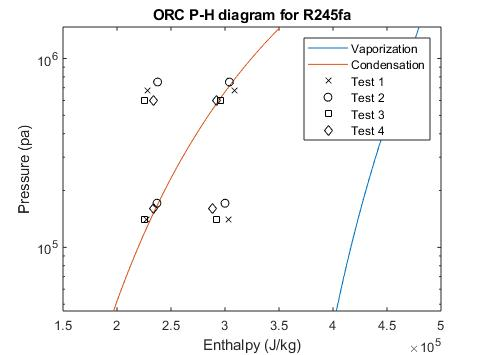
\includegraphics[width=\textwidth]{figures/VerificationPH01}
	%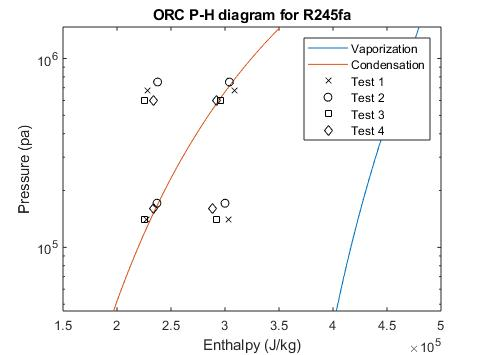
\includegraphics{figures/VerificationPH01}

	\caption{Pressure-Enthalpy plot of R245-fa for ORC verification. 
	For tests 1 \& 2 $T_{source}$ is about \SI{364}{\kelvin} (\SI{195}{\degreeFahrenheit})
	while for 3 \& 4 $T_{source}$ is \SI{353}{\kelvin} (\SI{175}{\degreeFahrenheit}). 
	In all cases $T_{sink}$ is about \SI{283}{\kelvin} (\SI{50}{\degreeFahrenheit}). 
	The hot water flow rate for tests 1 \& 3 are \SI{18.9}{\liter\per\second} (\SI{300}{\gpm})
	and	\SI{7.6}{\liter\per\second} (\SI{120}{\gpm}) for test 2 \& 4. 
	The cold water flow rate for tests 1 \& 3 are \SI{12.6}{\liter\per\second} (\SI{200}{\gpm})
	and \SI{7.6}{\liter\per\second} (\SI{120}{\gpm}) for test 2 \& 4.}
	\label{fig:verifcation_ph01}
\end{figure}
Pressure was plotted against enthalpy at various points of the cycle in \autoref{fig:verifcation_ph01} for each of the four tests. The two curves indicate the pressure-enthalpy combinations of R245-fa where the fluid begins to condense and vaporize. The top-left group of points represent the fluid at the outlet of the pump. The top-right group represent the fluid at the inlet of the expander. The bottom-right group represent the fluid at the outlet of the expander. Finally, The bottom-left group represent the fluid at the inlet of the pump.

For each of these tests, the fluid just barely begins to boil in the evaporator, if at all. It is expected that the fluid will either completely vaporize, or at least be further to the right in the liquid-vapor region. Along with the higher than expected pump power, this also indicates that there is more fluid being pumped along the cycle in the model than what was measured.

To re-create conditions where the system outputs comparable power while pumping less fluid, the evaporator area is increased by a factor of four so it is comparable to the area of the condenser. Additionally, the pressure set points are adjusted to values seen in \autoref{tab:verification_ORC_vars02} to account for the new temperatures of the working fluid.
\begin{table}%[h]
	\centering
	\caption{Input variables for the verification of the Organic Rankine Cycle Model.}
	%\rowcolors{5}{}{gray!10}
	\label{tab:verification_ORC_vars02}
	\begin{tabular}{rllll}
		\toprule
		                                              &  Case &       &       &       \\ \cline{2-5}
		                                              &     1 &     2 &     3 &     4 \\ \midrule

		$p_{hi}(\si{\kilo\pascal})  $                 &  0.68 &  0.75 &  0.60 &  0.60 \\
		$p_{low}(\si{\kilo\pascal}) $                 &  0.14 &  0.17 &  0.14 &  0.16 \\
%		$P_{setpoint}(\si{\kilo\watt})$               &  34.7 &  27.1 &  24.6 &  19.0 \\ 
		\bottomrule
	\end{tabular}
\end{table}



\autoref{tab:verification_results02} shows the new results verifications tests. As expected, the gross output power remained roughly equal to the measured values. The consumed pump power decreased significantly. The calculated power values are now about half the measured ones, indicating the fluid is moving at a slower rate. The thermal power measurements are now greater than the calculated values by about \SIrange{30}{80}{\kilo\watt} and the source and sink outlet temperatures are correspondingly higher and lower. \autoref{fig:verifcation_ph02} shows the lower mass flow rate of working fluid allows it to fully vaporize due to the larger transfer area of the evaporator. 
\begin{table}%[h]
	\centering
	\caption{Comparison of output variables for the verification of the ORC Model with modified evaporator area.}
	%\rowcolors{5}{}{gray!10}
	\label{tab:verification_results02}
	\begin{tabular}{rllllllll}
		\toprule
		                                           & Case  &       &       &       &       &       &       &       \\ \cline{2-9}
		                                           & 1     &       & 2     &       & 3     &       & 4     &       \\
		                                           & Meas. & Model & Meas. & Model & Meas. & Model & Meas. & Model \\ \midrule
		              $P_{gross}(\si{\kilo\watt})$ & 40.7  & 40.7  & 31.8  & 31.9  & 29.2  & 29.2  & 22.7  & 22.5  \\
		               $P_{pump}(\si{\kilo\watt})$ & 2.6   & 1.1   & 1.9   & 0.92  & 1.5   & 0.72  & 1.3   & 0.55  \\
		            %$P_{source}(\si{\kilo\watt})$ & 9.6   & -     & 1.0   & -     & 10.0  & -     & 1.0   & -     \\
		              %$P_{sink}(\si{\kilo\watt})$ & 3.5   & -     & 1.0   & -     & 3.5   & -     & 1.0   & -     \\
		              $P_{evap.}(\si{\kilo\watt})$ & 519   & 441   & 413   & 340   & 393   & 364   & 328   & 277   \\
		              $P_{cond.}(\si{\kilo\watt})$ & 464   & 400   & 385   & 307   & 356   & 335   & 303   & 254   \\
		            $T_{source,out}(\si{\kelvin})$ & 357.2 & 358.2 & 350.1 & 352.5 & 347.9 & 348.2 & 342.0 & 343.7 \\
		              $T_{sink,out}(\si{\kelvin})$ & 292.1 & 290.9 & 296.9 & 294.4 & 290.1 & 289.7 & 294.2 & 292.6 \\ \bottomrule
		          %$P_{setpoint}(\si{\kilo\watt})$ &       &       &       &       &       &       &       &       \\
		%$\dot{m}_{wf}(\si{\kilogram\per\second})$ & -     &       & -     &       & -     &       & -     &
	\end{tabular}
\end{table}


\begin{figure}%[h]
	\centering
	\caption{Pressure-Enthalpy plot of R245-fa for ORC verification with an over sized evaporator area. Input tempetures and flow rates remain the same. 
	For tests 1 \& 2 $T_{source}$ is about \SI{364}{\kelvin} (\SI{195}{\degreeFahrenheit})
	while for 3 \& 4 $T_{source}$ is \SI{353}{\kelvin} (\SI{175}{\degreeFahrenheit}). 
	In all cases $T_{sink}$ is about \SI{283}{\kelvin} (\SI{50}{\degreeFahrenheit}). 
	The hot water flow rate for tests 1 \& 3 are \SI{18.9}{\liter\per\second} (\SI{300}{\gpm})
	and	\SI{7.6}{\liter\per\second} (\SI{120}{\gpm}) for test 2 \& 4. 
	The cold water flow rate for tests 1 \& 3 are \SI{12.6}{\liter\per\second} (\SI{200}{\gpm})
	and \SI{7.6}{\liter\per\second} (\SI{120}{\gpm}) for test 2 \& 4.}
	\label{fig:verifcation_ph02}
	
	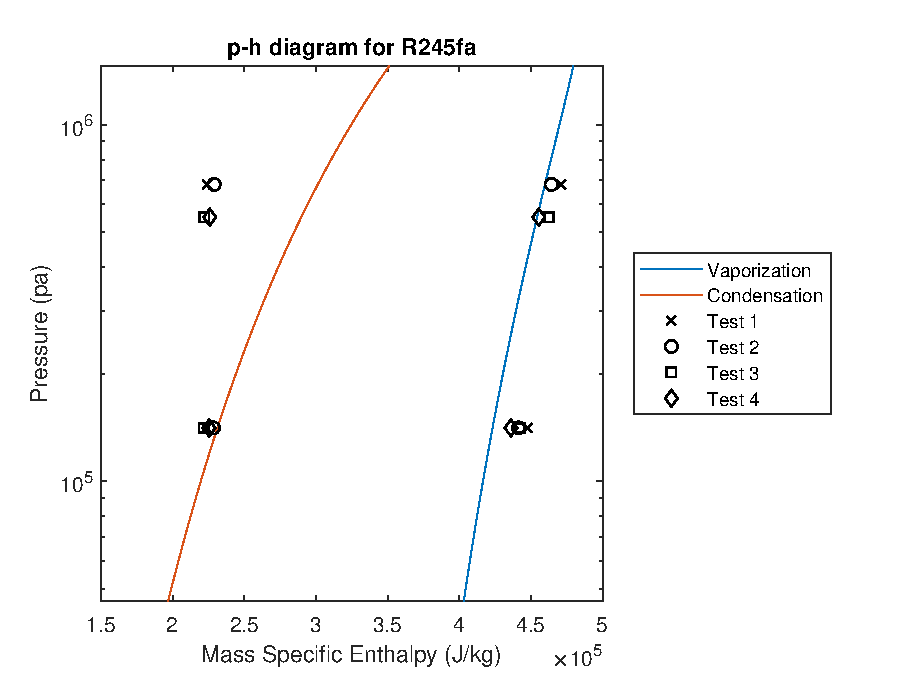
\includegraphics[width=\textwidth]{figures/VerificationPH02}
	%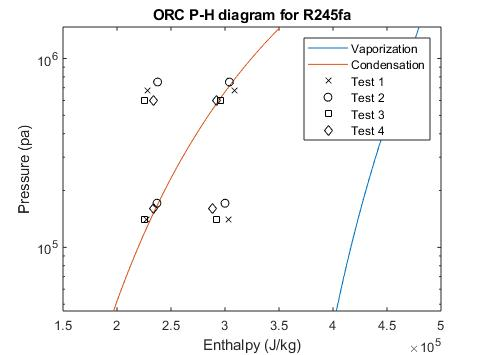
\includegraphics{figures/VerificationPH01}
\end{figure}